\documentclass{beamer}

% Theme choice
\usetheme{Boadilla}

% Packages
\usepackage{graphicx}
\usepackage[outputdir=build]{minted}
\usemintedstyle{manni}
\usepackage{tikz}
\usetikzlibrary{arrows.meta,calc,positioning,shapes.geometric}
\usepackage{pgfplots}
\pgfplotsset{compat=1.18} % A clean, colorful style
\setminted{fontsize=\small, breaklines, framesep=2mm}

% Title page details
\title{Mandelbrot Set Image Generation}
\subtitle{Maths, Data, and Machines}
\author{Gareth Lloyd}
\institute{ACCU York}
\date{2nd July 2025}

\begin{document}

% Title page
\begin{frame}
    \titlepage
\end{frame}

% Outline slide
\begin{frame}{Outline}
    \tableofcontents
\end{frame}

% Sections
\section{Introduction}
\begin{frame}{What is the Mandelbrot Set?}
    \begin{itemize}
        \item A famous mathematical set of complex numbers
        \item Boundary forms a fractal pattern
        \item High-quality visualization made by Benoit Mandelbrot in 1980
        \item First defined and drawn by Robert W. Brooks and Peter Matelski in 1978
        \item Generated by iterating a simple mathematical formula
    \end{itemize}
\end{frame}

\section{Generating the Image}
\begin{frame}{The Mathematical Foundation}

    \begin{block}{The Mandelbrot Formula}
        $z_{n+1} = z_n^2 + c$
    \end{block}
    \begin{itemize}
        \item Starting with $z_0 = 0$
        \item $c$ is a point in the complex plane
        \item If the sequence remains bounded, the point is in the set
        \item A sequence diverges to infinity if $|z_n| > 2$, hence iteration can be stopped
    \end{itemize}
\end{frame}

\begin{frame}{Complex Numbers}
    \begin{columns}
        \begin{column}{0.5\textwidth}
            \begin{tikzpicture}[scale=1.2,>=Stealth]
                % Axes
                \draw[->,thick] (-0.5,0) -- (4,0) node[below] {Real};
                \draw[->,thick] (0,-0.5) -- (0,3) node[left] {Imaginary};
                
                % Grid
                \draw[gray!30] (-0.5,-0.5) grid (3.5,2.5);
                
                % Point z = a + bi
                \coordinate (z) at (2.5,1.5);
                \filldraw[blue] (z) circle (1.5pt) node[above right] {$z = a + bi$};
                \draw[dashed] (2.5,0) node[below] {$a$} -- (z) -- (0,1.5) node[left] {$bi$};
                \draw[->,thick,red] (0,0) -- (z);
                \draw (1.0,0.9) node[rotate=31] {$|z| = \sqrt{a^2 + b^2}$};
            \end{tikzpicture}
        \end{column}
        \begin{column}{0.45\textwidth}
            \begin{itemize}
                \item Complex number $z = a + bi$
                \item $a$: real part (x-axis)
                \item $b$: imaginary part (y-axis)
                \item $|z| = \sqrt{a^2 + b^2}$: magnitude
                \item $i^2 = -1$
            \end{itemize}
        \end{column}
    \end{columns}
\end{frame}

\begin{frame}[fragile]{Algorithm Overview}
    \begin{enumerate}
        \item Choose a region in the complex plane
        \item For each pixel:
        \begin{itemize}
            \item Map to complex number $c$
            \item Iterate the formula
            \item Color based on escape time (number of iterations)
        \end{itemize}
    \end{enumerate}
\end{frame}

\begin{frame}{Mandelbrot Set Visualization}
    \begin{center}
        
\includegraphics[width=0.8\textwidth]{images/mandelbrot_set_1.jpg}
        \\[0.5em]
        \footnotesize Image by Wolfgang Beyer (CC BY-SA 3.0)
    \end{center}
\end{frame}

\section{Optimization Journey}
\begin{frame}[fragile]{Naïve}
    \begin{block}{Using std::complex}
        \begin{itemize}
            \item Clean, readable code using standard library
            \item \texttt{std::complex} handles complex arithmetic
            \item Easy to understand and maintain
        \end{itemize}
    \end{block}
    \begin{exampleblock}{Implementation}
        \begin{minted}[fontsize=\tiny,baselinestretch=0.8]{cpp}
auto mandelbrot(std::complex<double> c) -> std::size_t {
  auto iter = std::size_t{};
  auto z = std::complex<double>{};
  
  while (std::abs(z) <= 2.0 and iter < MAX_ITER) {
    z = z * z + c;
    ++iter;
  }
  return iter;
}
        \end{minted}
    \end{exampleblock}
\end{frame}

\begin{frame}{Engineering Mindset}
    \begin{block}{Evidence-Driven Development}
        \begin{itemize}
            \item Avoid premature optimization based on assumptions
            \item Let evidence guide your efforts
            \item Similar to TDD: Know when something is wrong because the tests fail
        \end{itemize}
    \end{block}
    \begin{exampleblock}{Performance Optimization Cycle}
        \begin{enumerate}
            \item Profile and measure current performance
            \item Identify actual bottlenecks (not assumed ones)
            \item Make targeted improvements
            \item Verify with measurements
            \item Repeat
        \end{enumerate}
    \end{exampleblock}
\end{frame}

\begin{frame}[fragile]{Benchmarking Setup}
    \begin{exampleblock}{Google Benchmark Code}
        \begin{minted}[fontsize=\tiny,baselinestretch=0.8]{cpp}
static void BM_Mandelbrot_V1(benchmark::State &state) {
  for (auto _ : state) {
    auto result = mandelbrot<MAX_ITER>(std::complex{0.0, 0.0});
    benchmark::DoNotOptimize(result);
  }
  state.counters["calc"] = benchmark::Counter(1, benchmark::Counter::kIsIterationInvariantRate);
}
BENCHMARK(BM_Mandelbrot_V1);
        \end{minted}
    \end{exampleblock}

    \begin{block}{Profiling Tools}
        \begin{itemize}
            \item Google Benchmark for microbenchmarking
            \item Linux \texttt{perf} for performance analysis
            \item \texttt{Hotspot} as a convenient GUI for \texttt{perf}
        \end{itemize}
    \end{block}

    \begin{block}{Why 0.0 + 0.0i?}
        \begin{itemize}
            \item This is the worst case, it is in the set and can not escape
            \item Are there other cases we should profile?
        \end{itemize}
    \end{block}
\end{frame}

\begin{frame}{Performance Analysis}
    \begin{center}
        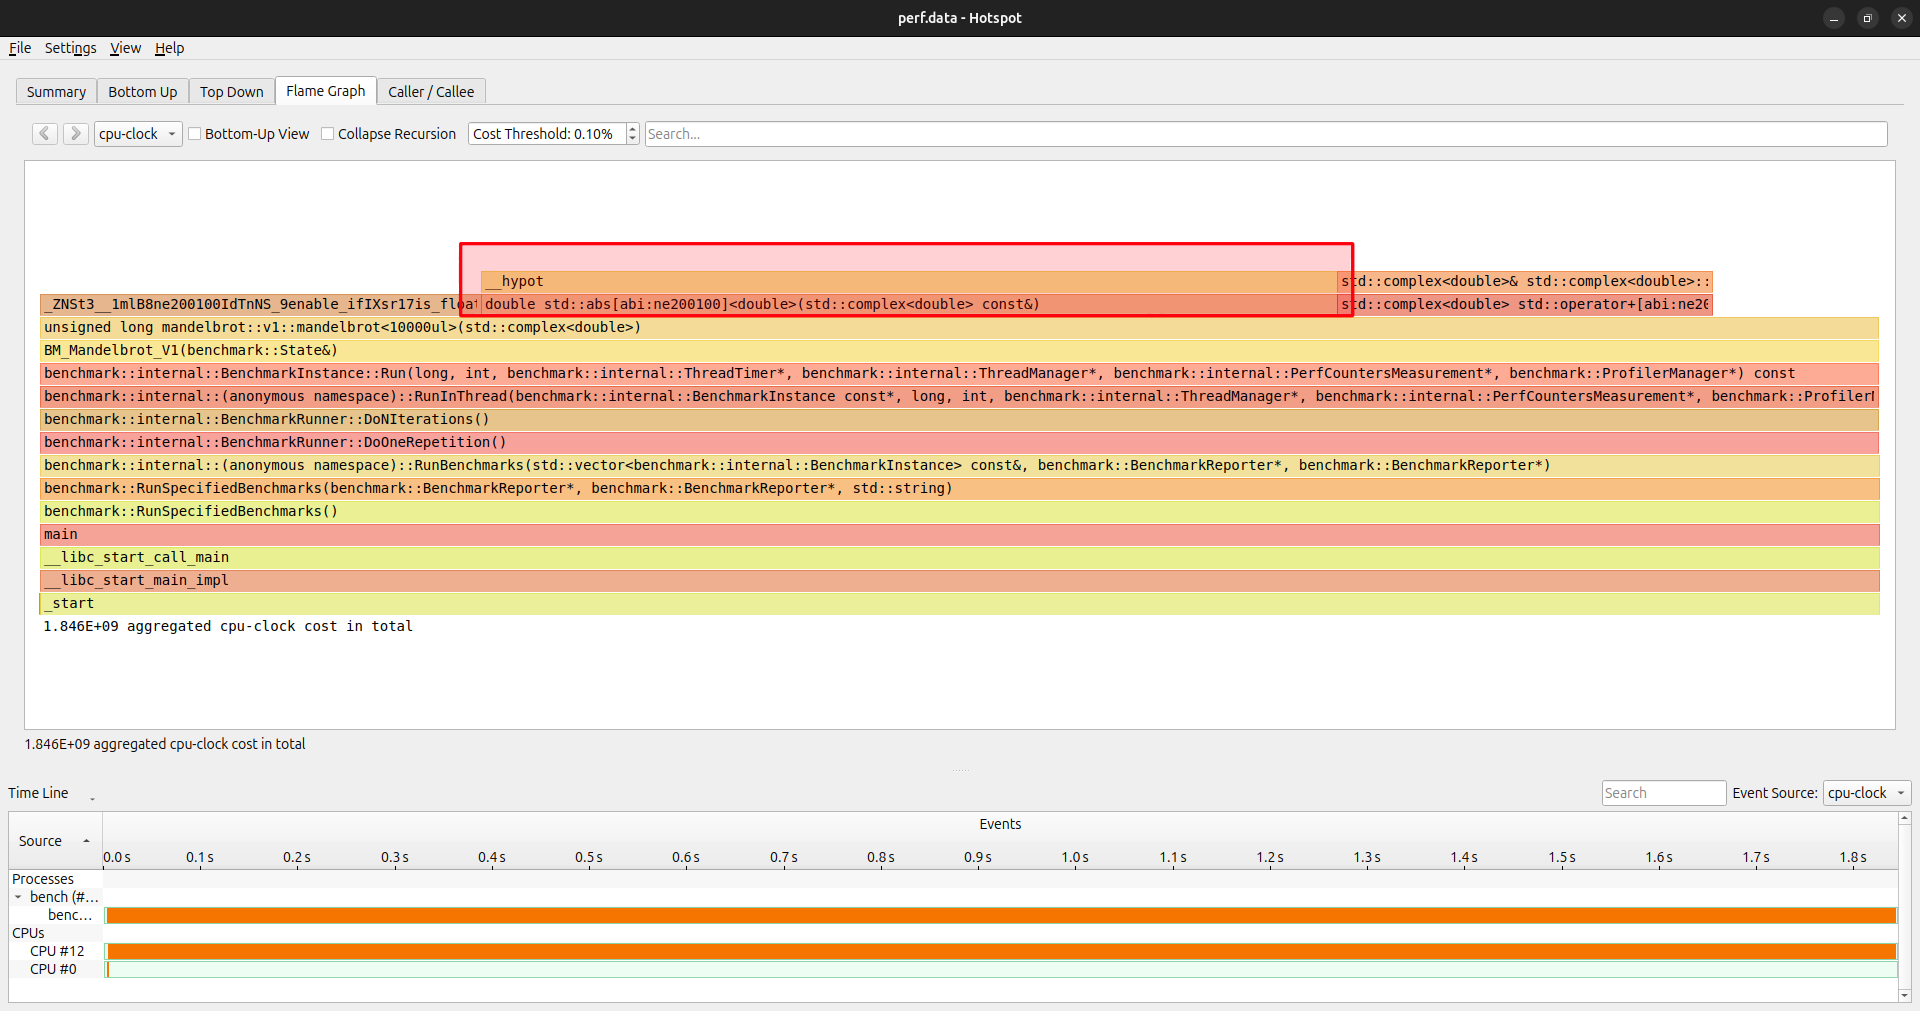
\includegraphics[width=0.9\textwidth]{images/V1_perf.png}
    \end{center}
    \begin{itemize}
        \item Profiling reveals significant time spent in \texttt{std::abs()}
    \end{itemize}
\end{frame}

\begin{frame}{The Problem with \texttt{std::abs}}
    \begin{block}{Performance Issues}
        \begin{itemize}
            \item \texttt{std::abs} for \texttt{std::complex} calls \texttt{\_\_hypot}
            \item \texttt{\_\_hypot} is a non-inlinable C library call
            \item \texttt{\_\_hypot} internally performs an expensive square root operation
        \end{itemize}
    \end{block}
    
    \begin{block}{Mathematical Insight}
        \begin{minipage}{\linewidth}
        \begin{align*}
            \mathrm{hypot}(z) \le 2 &\Leftrightarrow \sqrt{a^2 + b^2} \le 2 \\
                                    &\Leftrightarrow a^2 + b^2 \le 4 \\
                                    &\Leftrightarrow \mathrm{norm}(z) \le 4
        \end{align*}
        \end{minipage}
    \end{block}
    

\end{frame}

\begin{frame}[fragile]{Optimized}
    \begin{block}{Using std::norm}
        \begin{itemize}
            \item Replaces \texttt{std::abs(z) <= 2} with \texttt{std::norm(z) <= 4}
            \item Avoids expensive square root operation, maintains mathematical equivalence
        \end{itemize}
    \end{block}
    \begin{exampleblock}{Implementation}
        \begin{minted}[fontsize=\tiny,baselinestretch=0.8]{cpp}
auto mandelbrot(std::complex<double> c) -> std::size_t {
  auto iter = std::size_t{};
  auto z = std::complex<double>{};
  
  while (std::norm(z) <= 4.0 and iter < MAX_ITER) {
    z = z * z + c;
    ++iter;
  }
  return iter;
}
        \end{minted}
    \end{exampleblock}
\end{frame}

\begin{frame}{Performance Analysis}
    \begin{center}
        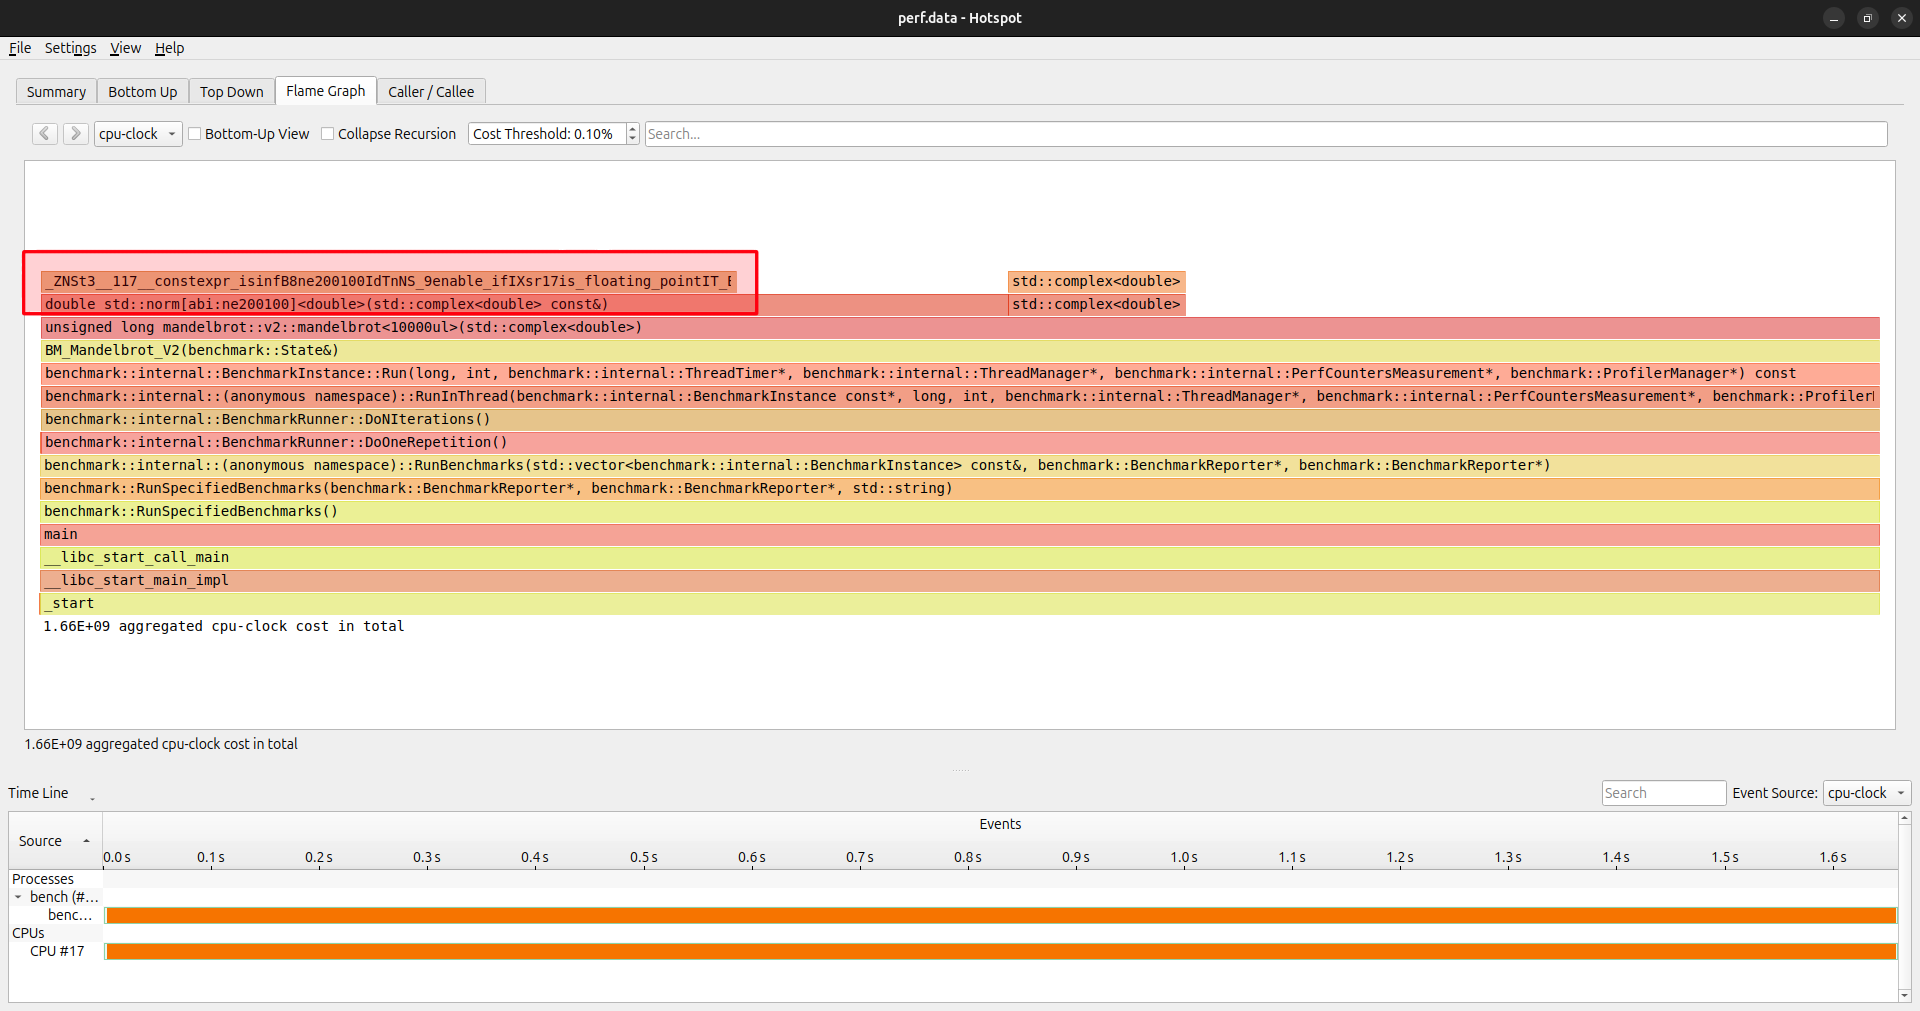
\includegraphics[width=0.9\textwidth]{images/V2_perf.png}
    \end{center}
    \begin{itemize}
        \item Small amount of work to handle infinities
        \item Our values stay small we don't need to handle infinities
    \end{itemize}
\end{frame}

\begin{frame}[fragile]{Manual}
    \begin{block}{Avoiding \texttt{std::norm}}
        \begin{itemize}
            \item Directly compute $x^2 + y^2$ instead of using \texttt{std::norm}
            \item No need to handle special cases (infinities, NaNs)
            \item More explicit control over the computation
        \end{itemize}
    \end{block}

    \begin{exampleblock}{Implementation}
        \begin{minted}[fontsize=\tiny,baselinestretch=0.8]{cpp}
auto mandelbrot(std::complex<double> c) -> std::size_t {
  auto iter = std::size_t{};
  auto z = std::complex<double>{};

  auto not_escaped = [](std::complex<double> z) {
    auto x = z.real();
    auto y = z.imag();
    return x * x + y * y <= 4.0;
  };

  while (not_escaped(z) and iter < MAX_ITER) {
    z = z * z + c;
    ++iter;
  }
  return iter;
}
        \end{minted}
    \end{exampleblock}
\end{frame}

\begin{frame}{Performance Analysis}
    \begin{center}
        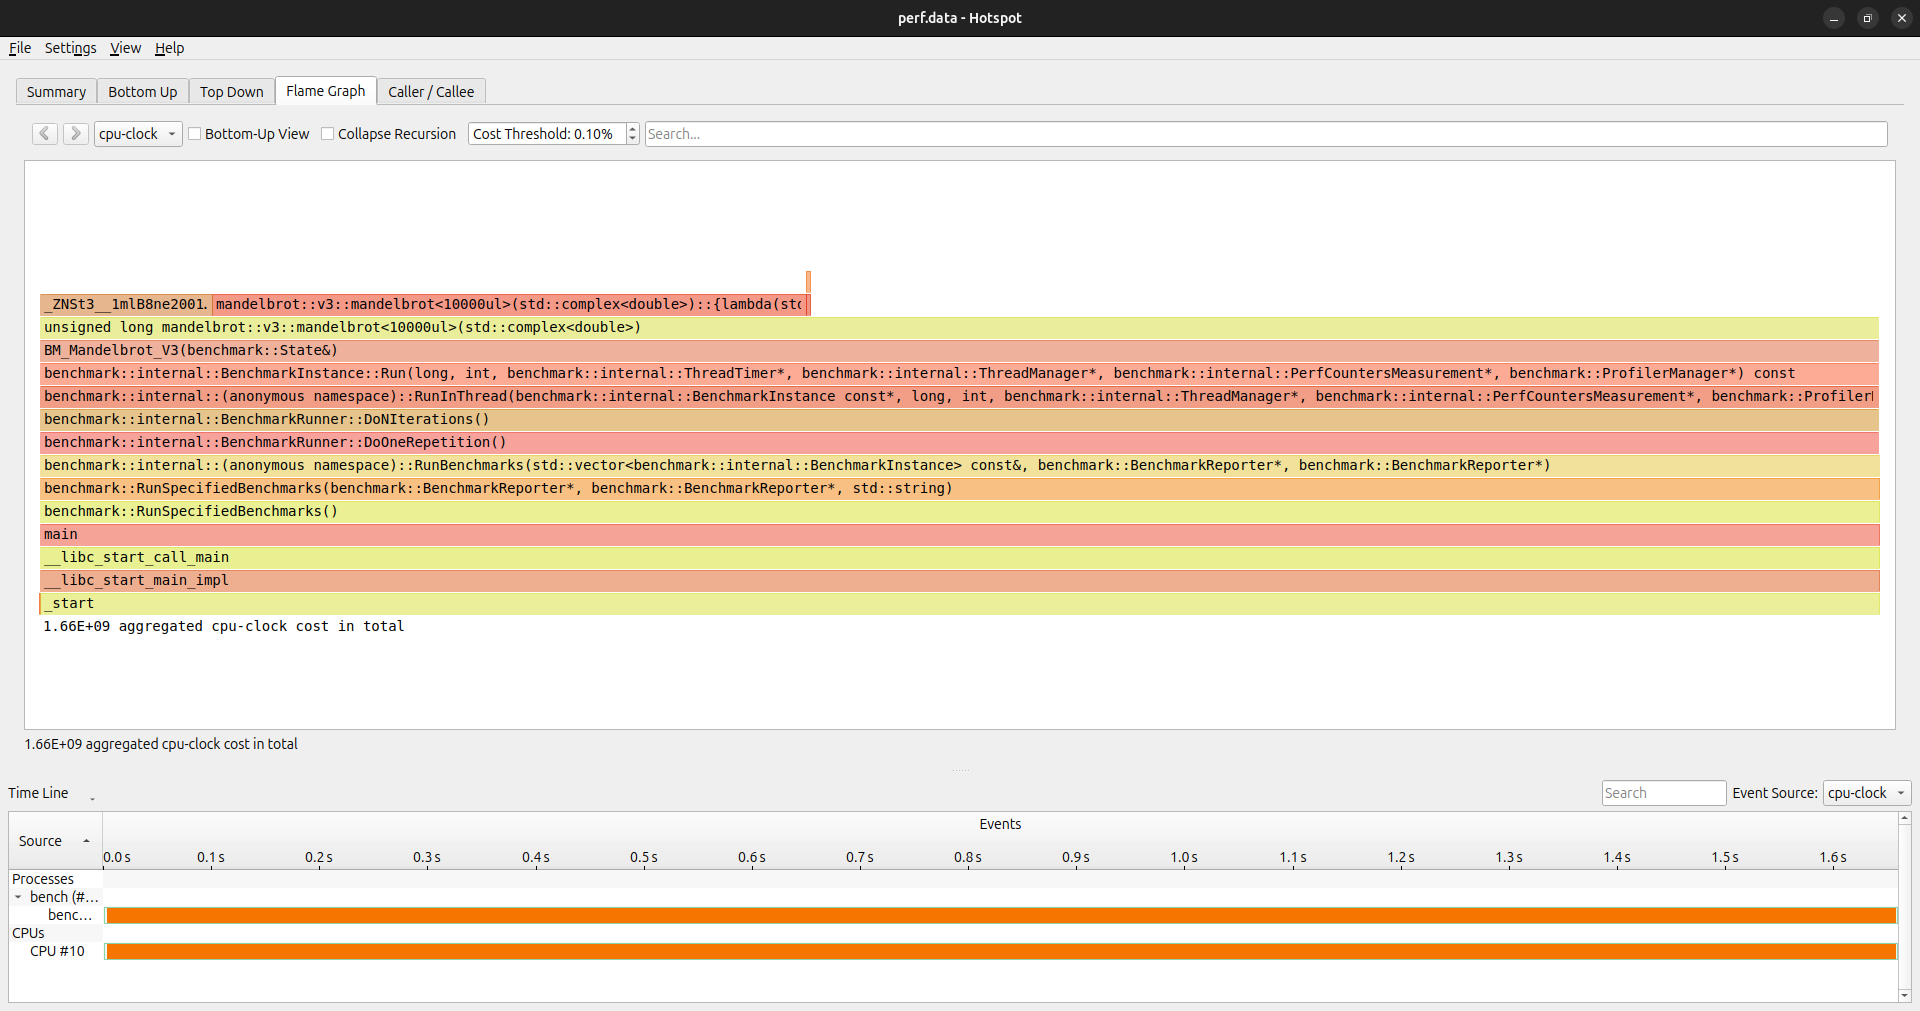
\includegraphics[width=0.9\textwidth]{images/V3_perf.png}
    \end{center}
    \begin{itemize}
        \item Both implementations have nearly identical performance
        \item \texttt{std::norm} templated code is fully inlined by the compiler
    \end{itemize}
\end{frame}

\begin{frame}{Removing Abstractions}
    \begin{block}{Why Remove \texttt{std::complex}?}
        \begin{itemize}
            \item Potential overhead from abstraction
            \item Want explicit control over operations
            \item Better optimization opportunities
        \end{itemize}
    \end{block}
    \begin{block}{Mathematical Derivation}
    \small
    Starting with $z = x + yi$ and $c = a + bi$:
        \begin{align}
        z^2 + c 
        &= (x + yi)^2 + (a + bi) \nonumber\\
        &= (x^2 + 2xyi + (yi)^2) + (a + bi) \nonumber\\
        &= (x^2 + 2xyi + y^2i^2) + (a + bi) \nonumber\\
        &= (x^2 + 2xyi - y^2) + (a + bi) \quad \text{since } i^2 = -1 \nonumber\\
        &= x^2 + 2xyi - y^2 + a + bi \nonumber\\
        &= x^2 - y^2 + a + 2xyi + bi \nonumber\\
        &= (x^2 - y^2 + a) + i(2xy + b) \nonumber
        \end{align}
    \end{block}
    
    \begin{block}{Benefits}
        \begin{itemize}
            \item Eliminates \texttt{std::complex} abstraction
            \item Direct computation of real and imaginary parts
            \item More explicit control over operations
        \end{itemize}
    \end{block}
\end{frame}

\begin{frame}[fragile]{No Abstraction}
    \begin{exampleblock}{Implementation}
        \begin{minted}[fontsize=\tiny,baselinestretch=0.8]{cpp}
auto mandelbrot(std::complex<double> c) -> std::size_t {
  auto const a = c.real();
  auto const b = c.imag();
  auto iter = std::size_t{};
  auto x = 0.0;
  auto y = 0.0;
  
  while (x * x + y * y <= 4.0 and iter < MAX_ITER) {
    auto x_next = x * x - y * y + a;
    auto y_next = 2 * x * y + b;
    std::tie(x, y) = std::tie(x_next, y_next);
    ++iter;
  }
  return iter;
}
        \end{minted}
    \end{exampleblock}
    
    \begin{block}{Details}
        \begin{itemize}
            \item Uses \texttt{std::tie} for clean value updates
            \item Avoids temporary complex number objects
            \item Easier for compiler to see operation dependencies
            \item Better quality codegen, is faster
        \end{itemize}
    \end{block}
\end{frame}

\begin{frame}[fragile]{Computation Reuse}
    \begin{block}{Key Insight / Experiment}
        \begin{itemize}
            \item $x^2$ and $y^2$ are used in both the escape check and value update
            \item We can compute them once per iteration and reuse them
            \item Reduces redundant multiplications
        \end{itemize}
    \end{block}
    \begin{exampleblock}{Optimized Implementation}
        \begin{minted}[fontsize=\tiny,baselinestretch=0.8]{cpp}
auto mandelbrot(std::complex<double> c) -> std::size_t {
  auto const a = c.real();
  auto const b = c.imag();
  auto iter = std::size_t{};
  auto x = 0.0;
  auto y = 0.0;
  auto x2 = 0.0;  // x squared
  auto y2 = 0.0;  // y squared
  
  while (x2 + y2 <= 4.0 and iter < MAX_ITER) {
    auto x_next = x2 - y2 + a;
    auto y_next = 2 * x * y + b;
    std::tie(x, y) = std::tie(x_next, y_next);
    y2 = y * y;  // store to reuse in the loop check
    x2 = x * x;  // store to reuse in the loop check
    ++iter;
  }
  return iter;
}
        \end{minted}
    \end{exampleblock}
\end{frame}


\begin{frame}{Beyond Hotspot: Going Deeper with perf}
    \begin{block}{Hotspot's Limits}
        \begin{itemize}
            \item Hotspot was good for seeing the big picture, functions and lines of code
            \item Now we need instruction-level analysis
            \item Time to use Linux perf directly for detailed insights
        \end{itemize}
    \end{block}
    \begin{exampleblock}{Using perf assembly}
        \texttt{\# Record with call graph and debug info}\\
        \texttt{perf record -g --call-graph=dwarf ./bench \\}\\
        \texttt{\hspace{2em}--benchmark\_filter=BM\_Mandelbrot\_V4/0 \\}\\
        \texttt{\hspace{2em}--benchmark\_min\_time=1s}
        
        \texttt{\# View annotated assembly}\\
        \texttt{perf annotate}
    \end{exampleblock}
\end{frame}


\begin{frame}{Assembly Comparison}
    \begin{columns}
        \begin{column}{0.45\textwidth}
            \centering
            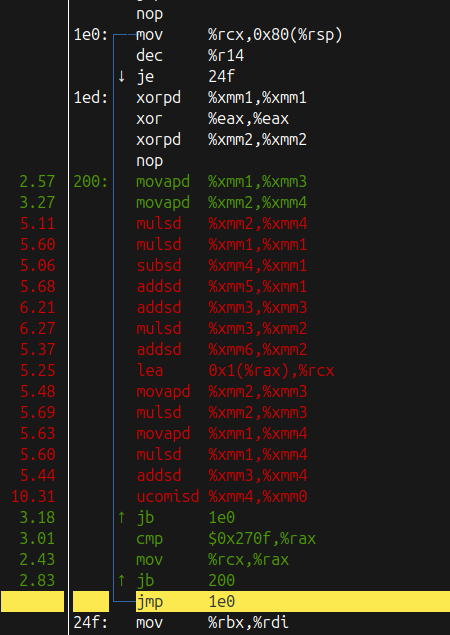
\includegraphics[width=0.9\textwidth,height=0.8\textheight,keepaspectratio]{images/V4_assembly_normal.png}
            \\
            \footnotesize No Abstraction
        \end{column}
        \hfill
        \begin{column}{0.45\textwidth}
            \centering
            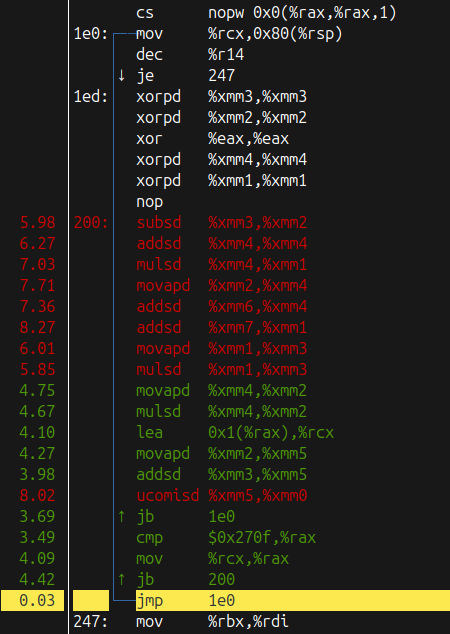
\includegraphics[width=0.9\textwidth,height=0.8\textheight,keepaspectratio]{images/V5_assembly_normal.png}
            \\
            \footnotesize Computation Reuse
        \end{column}
    \end{columns}
\end{frame}

\begin{frame}{Assembly Comparison}
    \begin{block}{Key Observations}
        \begin{itemize}
            \item Manual reuse can still be a beneficial optimization
            \begin{itemize}
                \item No abstraction: 4x moves, 5x multiplications, 6x add/subs
                \item Computation reuse: 4x moves, 3x multiplications, 6x add/subs
            \end{itemize}
            \item 2 fewer multiplications per iteration with reuse
            \item Manual optimization beneficial despite compiler optimizations
        \end{itemize}
    \end{block}
\end{frame}

\begin{frame}{Modern x86\_64 Microarchitecture Levels}
    \begin{block}{Our Current Code: Using x86\_64-v1 Instructions}
        \begin{itemize}
            \item Using \texttt{mulsd} (Multiply Scalar Double)
            \item Part of SSE2 (Streaming SIMD Extensions 2)
            \item Operates on just 2 registers at a time
        \end{itemize}
    \end{block}

    \begin{block}{x86\_64 Microarchitecture Levels}
        \begin{description}
            \item[x86\_64-v2] POPCNT, CMPXCHG16B
            \begin{itemize}
                \item Common since ~2011 (Nehalem/Bulldozer)
            \end{itemize}
            
            \item[x86\_64-v3] AVX, AVX2, BMI1/2, FMA, LZCNT
            \begin{itemize}
                \item Common since ~2015 (Haswell/Excavator)
            \end{itemize}
        \end{description}
    \end{block}
\end{frame}

\begin{frame}{Modern Compiler Targeting}
    \begin{block}{CMake Configuration}
        \texttt{target\_compile\_options(}\\
        \texttt{~~~~bench PRIVATE -march=x86-64-v3 -mtune=native}\\
        \texttt{)}
    \end{block}

    \begin{block}{Why Target x86\_64-v3?}
        \begin{itemize}
            \item Realistic for today's deployments
            \item Enables vectorized operations (AVX/AVX2)
            \item Modern math instructions (FMA)
            \item Bit manipulation (BMI1/2)
            \item Better bit operations (LZCNT)
        \end{itemize}
    \end{block}
\end{frame}

\begin{frame}{Assembly Comparison x86\_64-v3}
    \begin{columns}
        \begin{column}{0.45\textwidth}
            \centering
            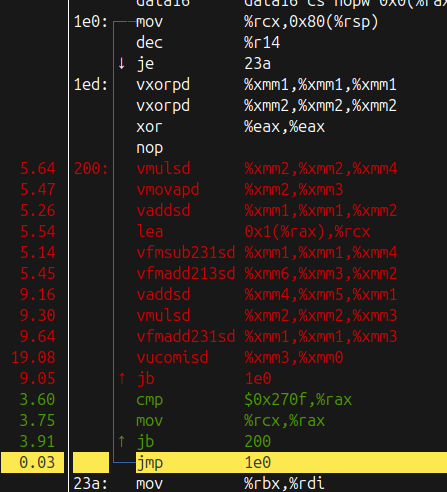
\includegraphics[width=0.9\textwidth,height=0.8\textheight,keepaspectratio]{images/V4_assembly_v3.png}
            \\
            \footnotesize No Abstraction
        \end{column}
        \hfill
        \begin{column}{0.45\textwidth}
            \centering
            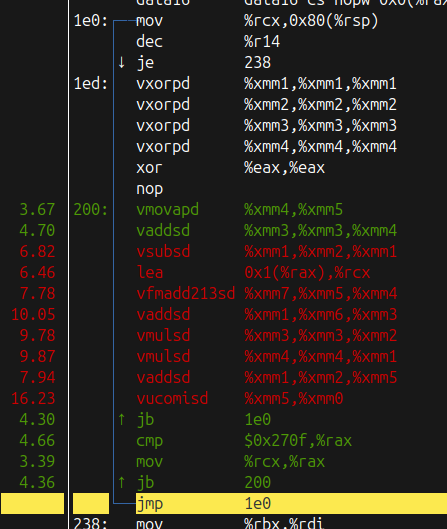
\includegraphics[width=0.9\textwidth,height=0.8\textheight,keepaspectratio]{images/V5_assembly_v3.png}
            \\
            \footnotesize Computation Reuse
        \end{column}
    \end{columns}
\end{frame}

\begin{frame}{Assembly Comparison x86\_64-v3}
    \begin{block}{Key Observations}
        \begin{itemize}
            \item Now the simpler code is faster, our computation reuse now hinders codegen
            \begin{itemize}
                \item No abstraction: 1x move, 2x multiplications, 3x add/subs 3x fma
                \item Computation reuse: 1x move, 2x multiplications, 5x add/subs, 1x fma
            \end{itemize}
            \item Not obvious why the simpler code is faster
            \item Sometimes KISS (keep it simple \& straightforward) is better
        \end{itemize}
    \end{block}
\end{frame}

\begin{frame}{Pipeline Analysis with LLVM-MCA}
    \begin{block}{What is LLVM-MCA?}
        \begin{itemize}
            \item A performance analysis tool that simulates CPU pipeline behavior
            \item Models out-of-order execution, register renaming, and instruction scheduling
            \item Helps identify pipeline stalls, port pressure, and bottlenecks
        \end{itemize}
    \end{block}
    
    \begin{exampleblock}{Why Use It?}
        \begin{itemize}
            \item Evidence driven approach to understand non-obvious performance differences
            \item Identifies resource contention and dependencies
            \item Helps understand the impact of instruction scheduling
            \item Particularly useful for analyzing microarchitecture-specific behavior
        \end{itemize}
    \end{exampleblock}
\end{frame}

\begin{frame}{LLVM-MCA Analysis}
    \begin{block}{Commands Used}
        \texttt{clang++-20 mandelbrot.cpp -std=c++23 -O3 -S -o - |} \\
        \texttt{~~~~llvm-mca-20 -mcpu=haswell}
    \end{block}
\end{frame}

\begin{frame}{LLVM-MCA Analysis}    
    \begin{block}{Results Comparison}
        \begin{tabular}{lrr}
            \textbf{Metric} & \textbf{No Abstraction} & \textbf{Computation Reuse} \\
            \hline
            Iterations & 100 & 100 \\
            Instructions & 1,900 & 2,100 \\
            Total Cycles & 572 & 621 \\
            Total uOps & 2,100 & 2,300 \\
            \hline
            uOps/Cycle & 3.67 & 3.70 \\
            IPC & 3.32 & 3.38 \\
            \textbf{Block RThroughput} & \textbf{5.3} & \textbf{5.8} \\
        \end{tabular}
    \end{block}
    
    \begin{alertblock}{Key Insight}
        The no-abstraction version has better (lower) Block RThroughput (5.3 vs 5.8), meaning it has better port scheduling and hence hides its latency better.
    \end{alertblock}
\end{frame}


\begin{frame}{What about SIMD?}
    \begin{block}{Single Instruction, Multiple Data}
        \begin{itemize}
            \item A parallel computing technique where one instruction operates on multiple data elements simultaneously
            \item Modern CPUs have dedicated SIMD instruction sets (SSE, AVX, AVX2, AVX-512)
            \item Perfect for operations on arrays, vectors, and mathematical computations
        \end{itemize}
    \end{block}
    
    \begin{block}{Benefits for Mandelbrot Generation}
        \begin{itemize}
            \item Calculate multiple results simultaneously
            \item Better utilization of CPU resources
            \item Mandelbrot is embarrassingly parallel
        \end{itemize}
    \end{block}
\end{frame}

\begin{frame}{Scalar Addition (Traditional)}
    \begin{center}
        \begin{tikzpicture}[scale=1.2]
            % Input arrays with color coding
            \foreach \i/\val/\color in {0/1.0/blue!30, 1/2.0/green!30, 2/3.0/orange!30, 3/4.0/purple!30} {
                \draw[fill=\color, thick] (\i*2, 4) rectangle ++(1.5, 0.8);
                \node at (\i*2+0.75, 4.4) {\Large\textbf{\val}};
            }
            \node[left] at (-0.5, 4.4) {\Large\textbf{A:}};
            
            \foreach \i/\val/\color in {0/5.0/blue!30, 1/6.0/green!30, 2/7.0/orange!30, 3/8.0/purple!30} {
                \draw[fill=\color, thick] (\i*2, 2.8) rectangle ++(1.5, 0.8);
                \node at (\i*2+0.75, 3.2) {\Large\textbf{\val}};
            }
            \node[left] at (-0.5, 3.2) {\Large\textbf{B:}};
            
            % Operations (4 separate additions) with color coding
            \foreach \i in {0, 1, 2, 3} {
%                 \draw[->, very thick, \color] (\i*2+0.75, 2.8) -- (\i*2+0.75, 2.0);
                \node at (\i*2+0.75, 2.4) {\Huge\textbf{\color{red}+}};
%                 \node at (\i*2+0.75, 2.4) {\Large\textbf{\color{red}+}};
            }
            
            % Results with color coding
            \foreach \i/\val/\color in {0/6.0/blue!30, 1/8.0/green!30, 2/10.0/orange!30, 3/12.0/purple!30} {
                \draw[fill=\color, thick] (\i*2, 1.2) rectangle ++(1.5, 0.8);
                \node at (\i*2+0.75, 1.6) {\Large\textbf{\val}};
            }
            \node[left] at (-0.5, 1.6) {\Large\textbf{C:}};
            
        \end{tikzpicture}
    \end{center}
    
    \begin{block}{Scalar Processing}
        \begin{itemize}
            \item 4 separate CPU instructions required
            \item Sequential execution
            \item One operation per clock cycle
        \end{itemize}
    \end{block}
\end{frame}

\begin{frame}{SIMD Addition (AVX2)}
    \begin{center}
        \begin{tikzpicture}[scale=1.2]
            % Input vectors with unified color coding
            \draw[fill=blue!20, thick] (0, 4) rectangle ++(8, 0.8);
            \foreach \i/\val in {0/1.0, 1/2.0, 2/3.0, 3/4.0} {
                \draw[thick] (\i*2, 4) -- (\i*2, 4.8);
                \node at (\i*2+1, 4.4) {\Large\textbf{\val}};
            }
            \node[left] at (-0.5, 4.4) {\Large\textbf{A:}};
            
            \draw[fill=green!20, thick] (0, 2.8) rectangle ++(8, 0.8);
            \foreach \i/\val in {0/5.0, 1/6.0, 2/7.0, 3/8.0} {
                \draw[thick] (\i*2, 2.8) -- (\i*2, 3.6);
                \node at (\i*2+1, 3.2) {\Large\textbf{\val}};
            }
            \node[left] at (-0.5, 3.2) {\Large\textbf{B:}};
            
            % Single operation arrow
            \node at (4, 2.4) {\Huge\textbf{\color{red}+}};
            \node[right] at (5, 2.4) {\large\color{red}\textbf{Single SIMD instruction}};
            
            % Result vector
            \draw[fill=orange!20, thick] (0, 1.2) rectangle ++(8, 0.8);
            \foreach \i/\val in {0/6.0, 1/8.0, 2/10.0, 3/12.0} {
                \draw[thick] (\i*2, 1.2) -- (\i*2, 2.0);
                \node at (\i*2+1, 1.6) {\Large\textbf{\val}};
            }
            \node[left] at (-0.5, 1.6) {\Large\textbf{C:}};
            
        \end{tikzpicture}
    \end{center}
    
    \begin{block}{SIMD Processing}
        \begin{itemize}
            \item Single CPU instruction (e.g., \texttt{vaddpd})
            \item Parallel execution within one instruction
            \item 4x theoretical speedup for this example
        \end{itemize}
    \end{block}
\end{frame}

\begin{frame}[fragile]{SIMD Mandelbrot Implementation}
    \begin{exampleblock}{xsimd-based Implementation}
        \begin{minted}[fontsize=\tiny,baselinestretch=0.8]{cpp}
auto mandelbrot(xsimd::batch<double> a, xsimd::batch<double> b)
    -> xsimd::batch<std::size_t> {
  using batch = xsimd::batch<double>;
  using bsize = xsimd::batch<std::size_t>;

  auto const four = batch(4.0);
  auto const two = batch(2.0);
  auto const one = bsize(1);

  auto x = batch(0.0);
  auto y = batch(0.0);
  auto iter = bsize(0);

  for (std::size_t i = 0; i < MAX_ITER; ++i) {
    auto const x2 = x * x;
    auto const y2 = y * y;

    auto const mask = (x2 + y2) <= four;
    if (none(mask)) {
      break;
    }

    auto const xy = x * y;
    auto const mask_i = batch_bool_cast<std::size_t>(mask);

    x = x2 - y2 + a;
    y = fma(two, xy, b);
    // Only update where still running
    iter = select(mask_i, iter + one, iter);
  }

  return iter;
}
        \end{minted}
    \end{exampleblock}
\end{frame}

\begin{frame}{SIMD Mandelbrot Key Concepts}
    \begin{block}{Processing Multiple Complex Numbers}
        \begin{itemize}
            \item \texttt{xsimd::batch<double>} gives largest size registers for your architecture, AVX2 would pack 4 doubles
            \item \texttt{mask = (x2 + y2) <= four} creates boolean mask for non-diverged points
            \item \texttt{select(mask, new\_value, old\_value)} conditionally updates only active points
            \item \texttt{if (none(mask))} early exit when all points have diverged
        \end{itemize}
    \end{block}
    
    \begin{block}{Performance Benefits}
        \begin{itemize}
            \item 4x theoretical speedup from processing 4 complex numbers simultaneously
            \item Efficient handling of divergence without branching
            \item Modern CPU features: FMA, efficient mask operations
        \end{itemize}
    \end{block}
\end{frame}

\begin{frame}{Intel Advisor for Performance Analysis}
    \begin{block}{What is Intel Advisor?}
        \begin{itemize}
            \item Performance profiling and optimization tool from Intel
            \item Provides vectorization analysis and roofline modeling
            \item Identifies optimization opportunities in CPU-bound applications
        \end{itemize}
    \end{block}

    \begin{center}
        \begin{tikzpicture}[scale=0.8]

            % Grid (lighter)
            \draw[gray!20] (0,0) grid[step=1] (7,4);

            % Axes
            \draw[->, thick] (0,0) -- (8,0);
            \draw[->, thick] (0,0) -- (0,5);
            
            % Axis labels
            \node[below] at (4,-0.3) {\small Operational Intensity [FLOP/byte]};
            \node[left, rotate=90] at (-0.4,4.5) {\small Performance [FLOP/s]};

            % Memory bandwidth roof (diagonal line)
            \draw[blue, very thick] (0.5,0.5) -- (3,3);

            % Compute roof (horizontal line)
            \draw[red, very thick] (3,3) -- (7,3);

            % Peak performance line
            \draw[red, dashed, thin] (0,3) -- (7,3);
            \node[above, red] at (1,3) {\tiny Peak FLOP/s};

            % Region labels
            \node[blue, rotate=45] at (1.6,2.1) {\small Memory Bound};
            \node[red] at (5,3.3) {\small Compute Bound};

            % Application points
            \filldraw[green!70!black] (1.2,1.2) circle (2pt);
            \node[green!70!black, right] at (1.2,1.2) {\tiny Mem-bound};

            \filldraw[orange] (5,3) circle (2pt);
            \node[orange, below] at (5,3) {\tiny Compute-bound};

            \filldraw[purple] (3.2,2.2) circle (2pt);
            \node[purple, right] at (3.2,2.2) {\tiny Some function};

        \end{tikzpicture}
    \end{center}

\end{frame}




\begin{frame}{Compare scalar to SIMD}

            \centering
            \includegraphics[width=0.95\textwidth]{images/V4_roofline.png}
            \\
            \footnotesize V4: No Abstraction (Scalar)


            \centering
            \includegraphics[width=0.95\textwidth]{images/V6_roofline.png}
            \\
            \footnotesize V6: SIMD Vectorization


\end{frame}


\begin{frame}{Possible extra SIMD Optimizations choices}
    \begin{block}{Loop Unrolling Strategies}
        \begin{itemize}
            \item \textbf{Reduced escape checking}: Check every 4, 8, or 16 iterations
            \item \textbf{Compiler hints}: \texttt{\#pragma clang loop unroll\_count(16)}
            \item \textbf{Benefit}: Reduces branch prediction penalties
        \end{itemize}
    \end{block}

    \begin{alertblock}{Is it worth it?}
        What is the likelihood of all members escaping?
        Are we ok to delay early exit by upto N-1 iterations?
    \end{alertblock}
\end{frame}

\begin{frame}[fragile]{SIMD with Loop Unrolling Implementation}
    \begin{exampleblock}{unrolled xsimd-based Implementation}
        \begin{minted}[fontsize=\tiny,baselinestretch=0.8]{cpp}
auto mandelbrot(xsimd::batch<double> a, xsimd::batch<double> b)
    -> xsimd::batch<std::size_t> {
  using batch = xsimd::batch<double>;
  using bsize = xsimd::batch<std::size_t>;

  auto const four = batch(4.0);
  auto const two = batch(2.0);
  auto const one = bsize(1);

  auto x = batch(0.0);
  auto y = batch(0.0);
  auto iter = bsize(0);

#pragma clang loop unroll_count(16)
  for (std::size_t i = 0; i < MAX_ITER; ++i) {
    auto const x2 = x * x;
    auto const y2 = y * y;

    auto const mask = (x2 + y2) <= four;
    if (i % 16 == 0 and none(mask)) {
      break;
    }

    auto const xy = x * y;
    auto const mask_i = batch_bool_cast<std::size_t>(mask);

    x = x2 - y2 + a;
    y = fma(two, xy, b);
    // Only update where still running
    iter = select(mask_i, iter + one, iter);
  }

  return iter;
}
        \end{minted}
    \end{exampleblock}
\end{frame}

\begin{frame}{Modern CPUs: Beyond Single Core}
    \begin{block}{The Multi-Core Reality}
        \begin{itemize}
            \item CPUs are no longer typically single core
            \item Even budget processors now have 4+ cores
            \item High-end consumer CPUs: 8-24+ cores
            \item Server CPUs: 64+ cores becoming common
        \end{itemize}
    \end{block}
    
    \begin{block}{Why Single-Threaded Limits Performance}
        \begin{itemize}
            \item Only utilizing 1/N of available CPU resources
            \item Mandelbrot calculation is embarrassingly parallel
            \item Each pixel calculation is independent
            \item Perfect candidate for multithreading
        \end{itemize}
    \end{block}
\end{frame}

\begin{frame}{Hardware Topology}
    \begin{center}
        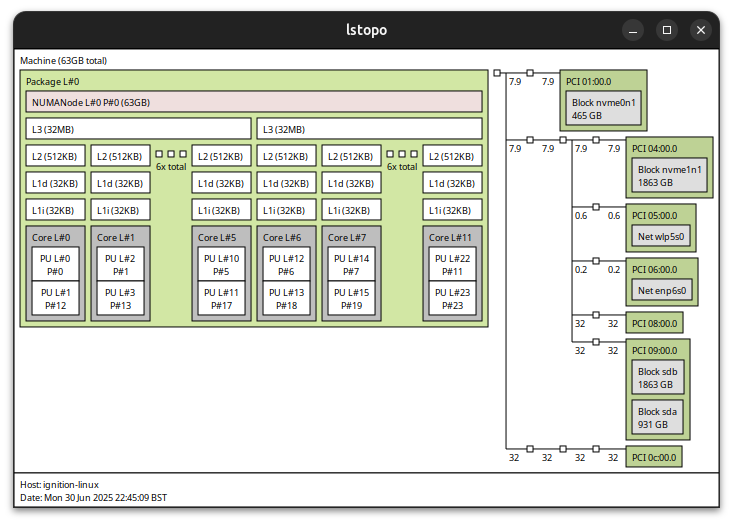
\includegraphics[width=0.9\textwidth]{images/lstopo.png}
    \end{center}
\end{frame}


\begin{frame}{Concurrent Overhead Visualization}
    \begin{center}
        \begin{tikzpicture}[scale=0.8]
            % Fine granularity (left)
%             \node[above] at (2,4.5) {\textbf{Fine Granularity}};
            \foreach \row in {0,1,2,3} {
                \foreach \col in {0,1,2,3} {
                    % Overhead squares (red border)
                    \draw[thick, red, fill=red!20] (\col*0.8, \row*0.8) rectangle (\col*0.8+0.7, \row*0.8+0.7);
                    % Useful work squares (smaller, green)
                    \draw[thick, green!70!black, fill=green!30] (\col*0.8+0.1, \row*0.8+0.1) rectangle (\col*0.8+0.6, \row*0.8+0.6);
                }
            }
            \node[below, red] at (1.5,0) {\small High Overhead};

            % Optimal granularity (center)
%             \node[above] at (6,4.5) {\textbf{Optimal Granularity}};
            \foreach \row in {0,1} {
                \foreach \col in {0,1} {
                    % Overhead squares (red border)
                    \draw[thick, red, fill=red!20] (4.5+\col*1.3, \row*1.3) rectangle (4.5+\col*1.3+1.2, \row*1.3+1.2);
                    % Useful work squares (much larger, green)
                    \draw[thick, green!70!black, fill=green!30] (4.5+\col*1.3+0.1, \row*1.3+0.1) rectangle (4.5+\col*1.3+1.1, \row*1.3+1.1);
                }
            }
            \node[below, green!70!black] at (4.5+1.3,0) {\small Low Overhead};

            % Coarse granularity (right)
%             \node[above] at (10,4.5) {\textbf{Coarse Granularity}};
            % Single large task
            \draw[thick, red, fill=red!20] (8.5, 0) rectangle (8.5+2.0+0.2, 2.0+0.2);
            \draw[thick, green!70!black, fill=green!30] (8.6, 0.1) rectangle (8.6+2.0, 2.1);
            % Idle threads
            \foreach \i in {0,1,2} {
                \draw[thick, gray, fill=gray!20] (8.5+\i*0.8, 2.5) rectangle (8.5+\i*0.8+0.7, 3.4);
                \node[gray] at (8.5+\i*0.8+0.35, 2.95) {\tiny Idle};
            }
            \node[below, orange] at (8.5+1.2,0) {\small Low Concurrency};
        \end{tikzpicture}
    \end{center}

    \begin{block}{Overhead vs Useful Work}
        \begin{itemize}
            \item \textcolor{red}{Red border}: Scheduling/synchronization/concurrency mechanism overhead
            \item \textcolor{green!70!black}{Green fill}: Useful computation work
        \end{itemize}
    \end{block}
\end{frame}

\begin{frame}{Thread Pool Task Scheduling}
    \begin{center}
        \begin{tikzpicture}[scale=1.0]
            % Task queue background
            \draw[thick, fill=blue!10] (-0.5,4.5) rectangle (4,6);
            \node[above] at (1.75,6) {\textbf{Task Queue}};
            
            % Individual tasks in queue
            \foreach \i in {0,1,2,3,4} {
                \draw[fill=blue!30, thick] (0.1+\i*0.7,4.7) rectangle (0.6+\i*0.7,5.8);
                \node at (0.35+\i*0.7,5.25) {\small T\i};
            }
            
            % Arrow from queue to scheduler
            \draw[->, thick, blue] (4,5.25) -- (4.8,5.25);
            
            % Thread pool scheduler (diamond shape)
            \node[diamond, draw, thick, fill=yellow!20, minimum width=2cm, minimum height=1cm] (scheduler) at (5.5,5.25) {\small\textbf{Scheduler}};
            
            % Thread pool container
            \draw[thick, fill=orange!10, dashed] (-0.5,2) rectangle (7,3.5);
            \node[above left] at (-0.5,3.5) {\textbf{Thread Pool}};
            
            % Worker threads
            \foreach \i in {0,1,2,3} {
                \draw[thick, fill=orange!20] (\i*1.6+0.2,2.2) rectangle (\i*1.6+1.4,3.3);
                \node at (\i*1.6+0.8,2.75) {\footnotesize Thread \i};
                
                % Arrow from scheduler to thread (from edge of diamond)
                \draw[->, thick, blue] (scheduler.south) -- (\i*1.6+0.8,3.3);
            }
            
            % Processing units container
            \draw[thick, fill=green!10, dashed] (-0.5,0) rectangle (7,1.5);
            \node[above left] at (-0.5,1.5) {\textbf{Processing Units}};
            
            % CPU cores
            \foreach \i in {0,1,2,3} {
                \draw[thick, fill=green!25] (\i*1.6+0.2,0.2) rectangle (\i*1.6+1.4,1.3);
                \node at (\i*1.6+0.8,0.75) {\small Core \i};
                
                % Arrow from thread to core
                \draw[->, thick, green!70!black] (\i*1.6+0.8,2.2) -- (\i*1.6+0.8,1.3);
            }
        \end{tikzpicture}
    \end{center}
\end{frame}

\begin{frame}[fragile]{Multithreaded SIMD Implementation}
    \begin{exampleblock}{stdexec-based Implementation}
        \begin{minted}[fontsize=\tiny,baselinestretch=0.8]{cpp}
void mandelbrot(std::vector<xsimd::batch<std::size_t>> &vec, 
                auto &&gen, auto scheduler) {
  auto sender = stdexec::bulk(
    stdexec::schedule(scheduler), 
    stdexec::par, 
    vec.size(), 
    [&](std::size_t i) {
      vec[i] = std::apply(mandelbrot_simd, gen(i));
    });

  stdexec::sync_wait(sender);
}
        \end{minted}
    \end{exampleblock}
    
    \begin{block}{Key Components}
        \begin{itemize}
            \item \textbf{stdexec::bulk}: Splits the work to be dones as multiple chunked tasks
            \item \textbf{stdexec::par}: Parallel execution policy
            \item \textbf{scheduler}: Dispatch + coordinate via a thread pool
            \item \textbf{gen(i)}: Generates coordinates for batch \texttt{i}
            \item \textbf{mandelbrot\_simd}: SIMD version from earlier
            \item \textbf{sync\_wait}: Waits for all tasks to complete
        \end{itemize}
    \end{block}
\end{frame}

\begin{frame}{Performance Results: Speedup vs Naive}
    \begin{block}{Individual Optimizations}
        \begin{itemize}
            \item Scalar optimizations: 1.8-2.2x improvement
            \item SIMD vectorization: 8-8.5x improvement
            \item Multithreading: 41x improvement (on 24 processing units)
            \item Combined MT + SIMD: \textbf{174x improvement}
        \end{itemize}
    \end{block}
\end{frame}

\section{Conclusion}
\begin{frame}{The Journey: From Maths to Machines}
    \begin{block}{Mathematical Foundation}
        \begin{itemize}
            \item Started with elegant mathematical formula: $z_{n+1} = z_n^2 + c$
            \item Explored the complex plane and fractal geometry
            \item Translated mathematical concepts into computational algorithms
        \end{itemize}
    \end{block}
    
    \begin{block}{Tools Gave Us Insight}
        \begin{itemize}
            \item \textbf{Profiling tools}: Hotspot, perf, Intel Advisor revealed bottlenecks
            \item \textbf{Assembly analysis}: Understanding what the compiler actually generates
            \item \textbf{LLVM-MCA}: Pipeline analysis for microarchitecture optimization
            \item \textbf{Benchmarking}: Evidence-driven development with Google Benchmark
        \end{itemize}
    \end{block}
\end{frame}

\begin{frame}{Understanding Your Platform}
    \begin{block}{Hardware Awareness Unlocks Performance}
        \begin{itemize}
            \item \textbf{CPU microarchitecture}: x86\_64-v3 enabled FMA and other better instructions
            \item \textbf{SIMD capabilities}: AVX2 provided 4x theoretical speedup, achieved 8.0x
            \item \textbf{Multi-core reality}: 24 processing units → 174x final speedup
        \end{itemize}
    \end{block}
    
    \begin{block}{Task Granularity is Critical}
        \begin{itemize}
            \item Too fine: Overhead dominates useful work
            \item Too coarse: Poor load balancing and resource waste
            \item Sweet spot: Balance between parallelism and scheduling costs
        \end{itemize}
    \end{block}
\end{frame}

\begin{frame}{The Learning Never Stops}
    \begin{block}{Technology Evolves Continuously}
        \begin{itemize}
            \item \textbf{Hardware changes}: New instruction sets, architectures, and capabilities
            \item \textbf{Languages evolve}: C++26 brings new abstractions (sender/receivers) [libstdexec]
            \item \textbf{Libraries advance}: xsimd provides portable SIMD, new algorithms emerge
        \end{itemize}
    \end{block}
    
    \begin{block}{Fundamental Principles Remain}
        \begin{itemize}
            \item Measure first, optimize second
            \item Understand your problem domain and hardware platform
            \item Balance abstraction with performance requirements
            \item Use tools to guide decisions, not assumptions
        \end{itemize}
    \end{block}
\end{frame}

\begin{frame}{Final Thoughts}
    \begin{exampleblock}{174x Speedup: The Journey Matters}
        \begin{itemize}
            \item Mathematical elegance → Clean initial implementation
            \item Profiling insights → Targeted optimizations (sqrt → norm)
            \item Assembly understanding → Manual improvements
            \item Hardware awareness → SIMD vectorization
            \item Platform knowledge → Effective multithreading
        \end{itemize}
    \end{exampleblock}
    
    \begin{block}{Keep Exploring}
        \begin{itemize}
            \item Try other fractal sets (Julia, Burning Ship, Newton)
            \item Experiment with GPU computing (CUDA, OpenCL, compute shaders)
            \item Explore distributed computing and cloud scaling
            \item Different coloring techniques
            \item Getting past IEEE double precision limits
        \end{itemize}
    \end{block}
\end{frame}

\end{document}
